\newcommand{\scoresAtMaxAccuracy}{
    \begin{table}[H]
        \centering
        \begin{tabular}{|P{2,8cm}||P{2,2cm} P{2,2cm} P{2,2cm} P{2,2cm}|}
            \hline
            & ALOHA\newline (M/B only) & ALOHA & Joint\newline Embedding & Proposed\newline Model \\
            \hline
            Accuracy & 0.299$\pm$0.048 & \textBF{0.398$\pm$0.051} & 0.273$\pm$0.058 & 0.223$\pm$0.044 \\
            Recall Micro & 0.299$\pm$0.048 & \textBF{0.398$\pm$0.051} & 0.273$\pm$0.058 & 0.223$\pm$0.044 \\
            Recall Macro & 0.299$\pm$0.048 & \textBF{0.398$\pm$0.051} & 0.273$\pm$0.058 & 0.223$\pm$0.044 \\
            Precision Micro & 0.299$\pm$0.048 & \textBF{0.398$\pm$0.051} & 0.273$\pm$0.058 & 0.223$\pm$0.044 \\
            Precision Macro & 0.295$\pm$0.093 & \textBF{0.465$\pm$0.056} & 0.291$\pm$0.088 & 0.154$\pm$0.055 \\
            f1 score Micro & 0.299$\pm$0.048 & \textBF{0.398$\pm$0.051} & 0.273$\pm$0.058 & 0.223$\pm$0.044 \\
            f1 score Macro & 0.248$\pm$0.050 & \textBF{0.386$\pm$0.054} & 0.216$\pm$0.062 & 0.147$\pm$0.042 \\
            AUC ROC Micro & 0.734$\pm$0.020 & \textBF{0.737$\pm$0.040} & 0.688$\pm$0.031 & 0.655$\pm$0.027 \\
            AUC ROC Macro & \textBF{0.750$\pm$0.023} & 0.736$\pm$0.043 & 0.711$\pm$0.034 & 0.689$\pm$0.035 \\
            \hline
            n. of anchors & 5 & 10 & 7 & 4 \\
            \hline
        \end{tabular}
        \caption[Family Prediction Scores at Maximum Accuracy]{Mean and standard deviation scores obtained by evaluating the different models on the Malware Family Prediction task with the number $k$ of anchors which produced the maximum accuracy (for each). Statistics were computed over 15 evaluation of the same models with different query and anchor samples. Best results are shown in \textbf{bold}.}
        \label{tab:ScoresAtMaxAccuracy}
    \end{table}
}

\newcommand{\allAccuracyTrends}{
    \begin{figure}[H]
        \vspace*{-0.5cm}
        \centering
        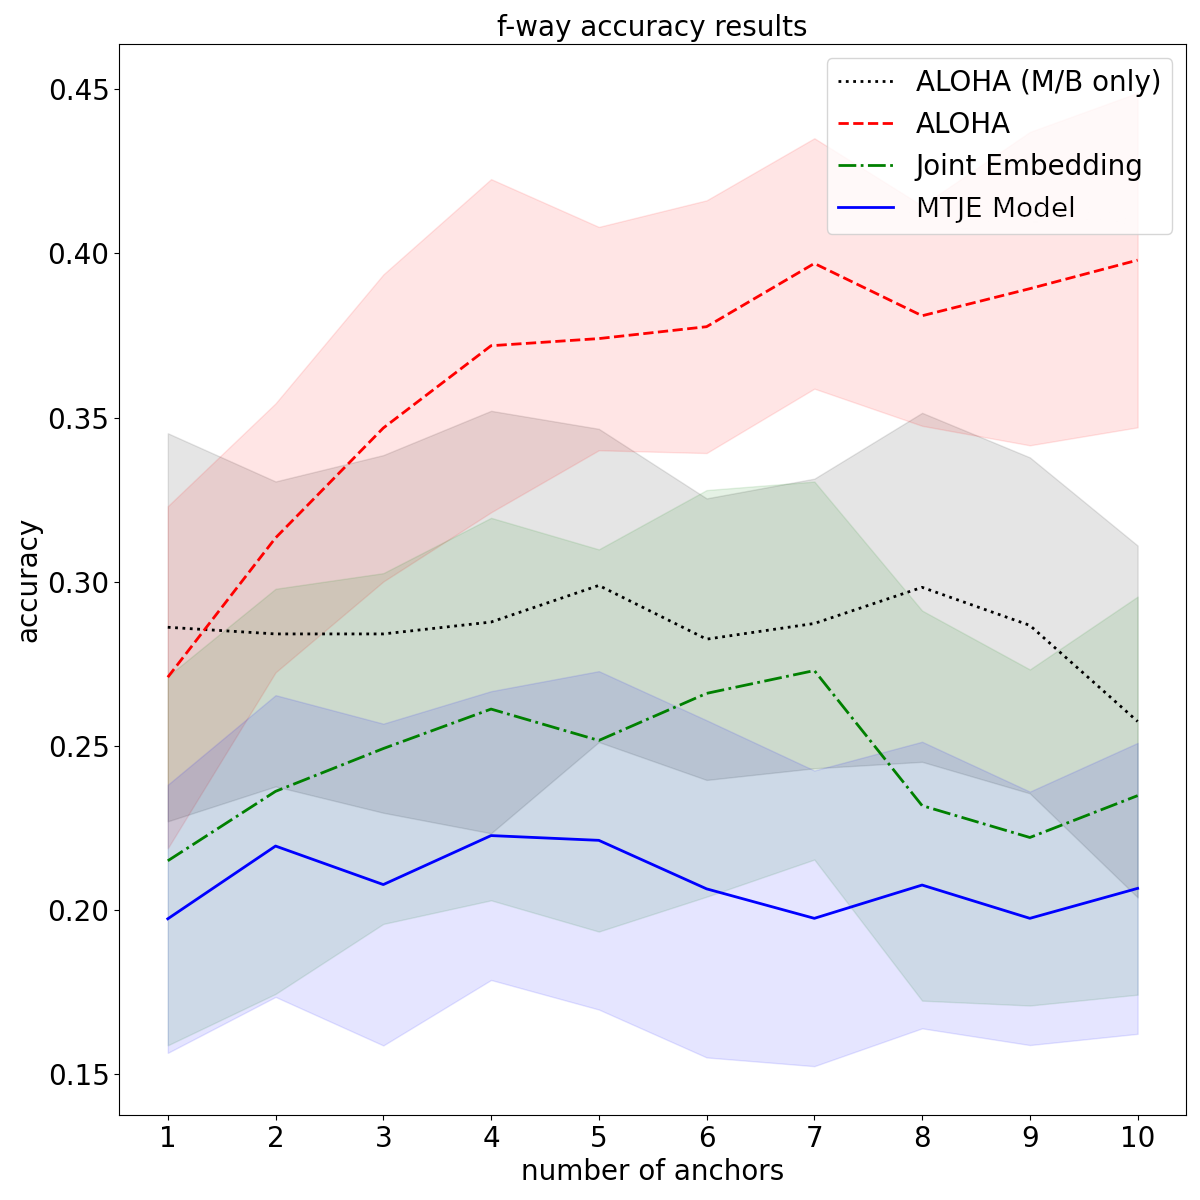
\includegraphics[width=0.7\textwidth]{./results/accuracy_trends.png}
        \vspace*{-0.2cm}
        \caption[Family Prediction Accuracy Trends]{\textBF{Accuracy Trend} (varying the number of anchor samples used) resulting from the evaluation of the different models on the Malware Family Prediction task. The line represents the \textit{mean} Accuracy, while the shaded region represents the \textit{standard deviation}. Statistics were computed over 15 evaluation of the same models with different query and anchor samples.}
        \label{fig:AccuracyTrends}
    \end{figure}
}

\newcommand{\allAucRocMacroTrends}{
    \begin{figure}[H]
        \vspace*{-0.5cm}
        \centering
        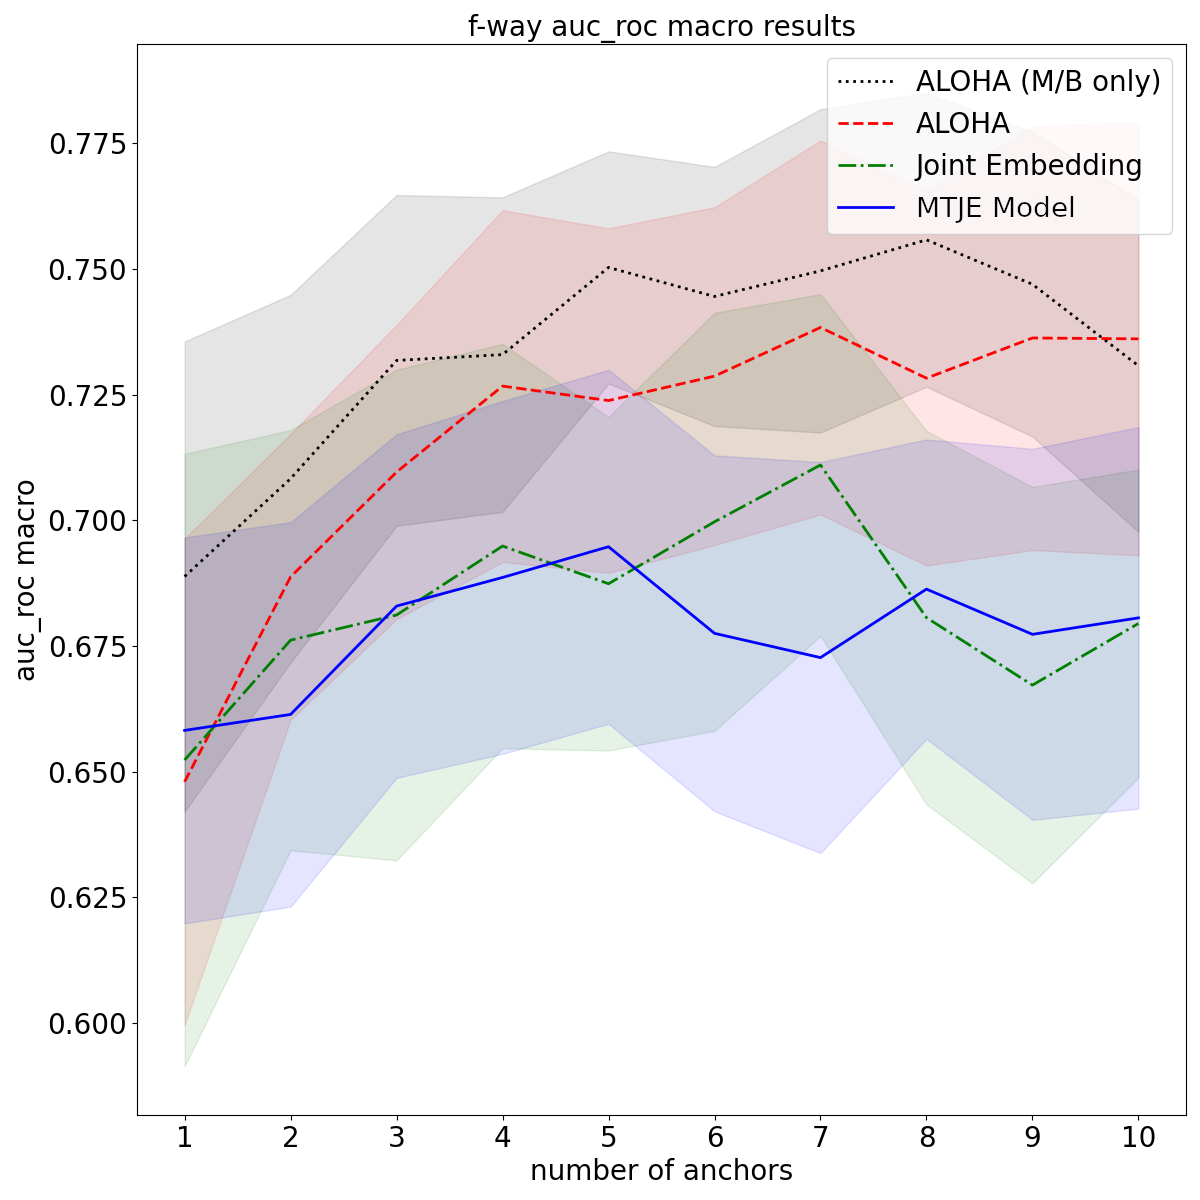
\includegraphics[width=0.7\textwidth]{./results/auc_roc_macro_trends.png}
        \vspace*{-0.2cm}
        \caption[Family Prediction AUC-ROC (Macro) Trends]{\textBF{AUC-ROC (Macro) Trend} (varying the number of anchor samples used) resulting from the evaluation of the different models on the Malware Family Prediction task. The line represents the \textit{mean} AUC-ROC (Macro), while the shaded region represents the \textit{standard deviation}. Statistics were computed over 15 evaluation of the same models with different query and anchor samples.}
        \label{fig:AucRocMacroTrends}
    \end{figure}
}

\newcommand{\allAucRocMicroTrends}{
    \begin{figure}[H]
        \vspace*{-0.5cm}
        \centering
        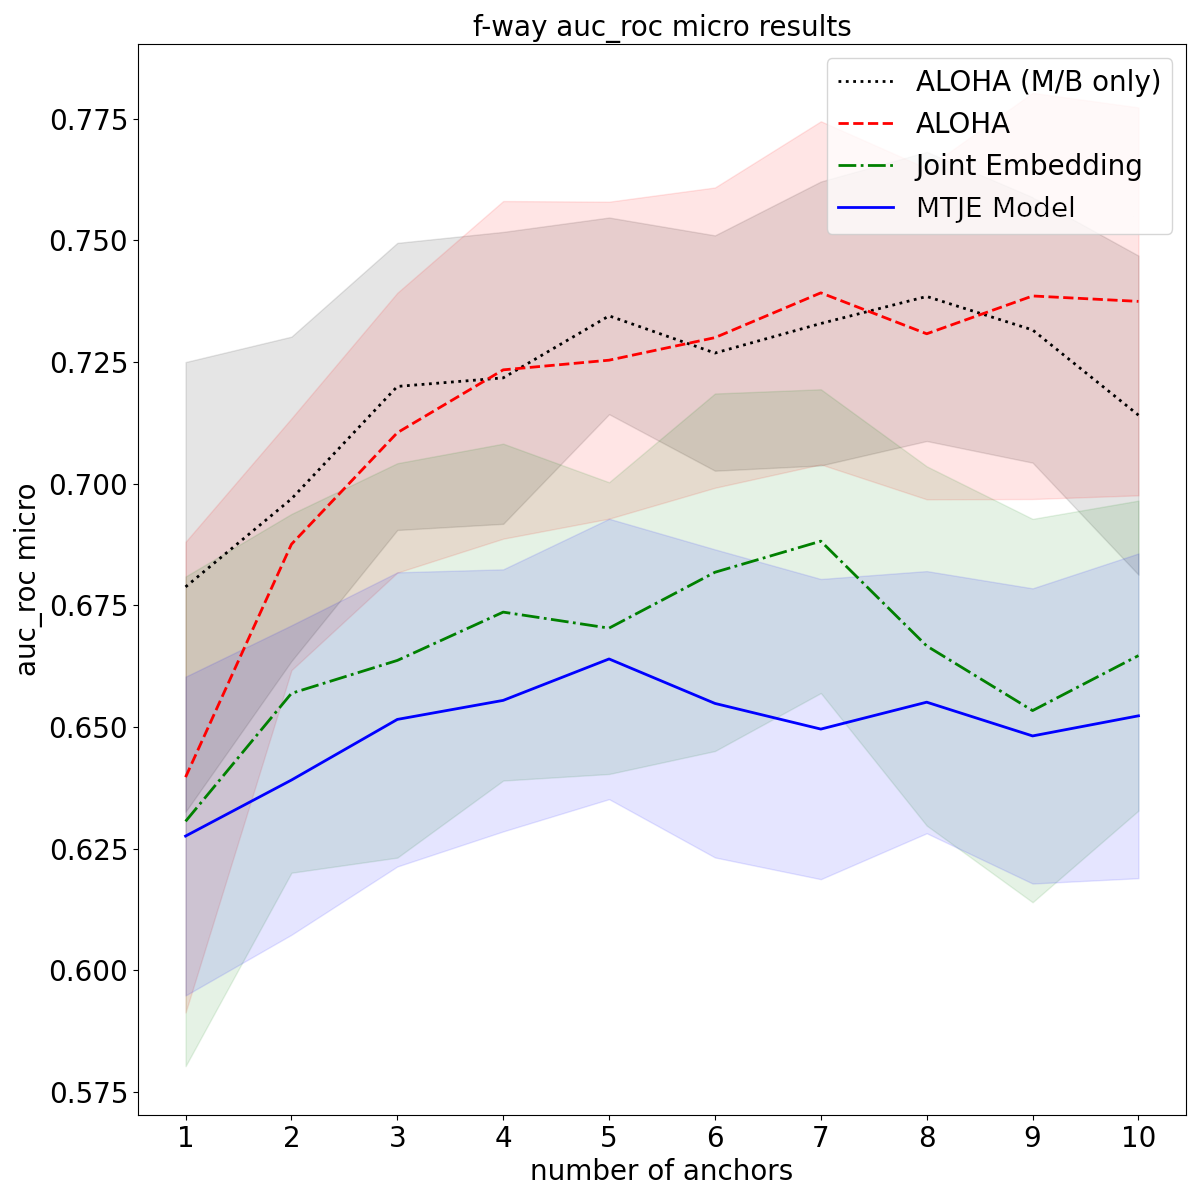
\includegraphics[width=0.7\textwidth]{./results/auc_roc_micro_trends.png}
        \vspace*{-0.2cm}
        \caption[Family Prediction AUC-ROC (Micro) Trends]{\textBF{AUC-ROC (Micro) Trend} (varying the number of anchor samples used) resulting from the evaluation of the different models on the Malware Family Prediction task. The line represents the \textit{mean} AUC-ROC (Micro), while the shaded region represents the \textit{standard deviation}. Statistics were computed over 15 evaluation of the same models with different query and anchor samples.}
        \label{fig:AucRocMicroTrends}
    \end{figure}
}

\newcommand{\allFScoreMacroTrends}{
    \begin{figure}[H]
        \vspace*{-0.5cm}
        \centering
        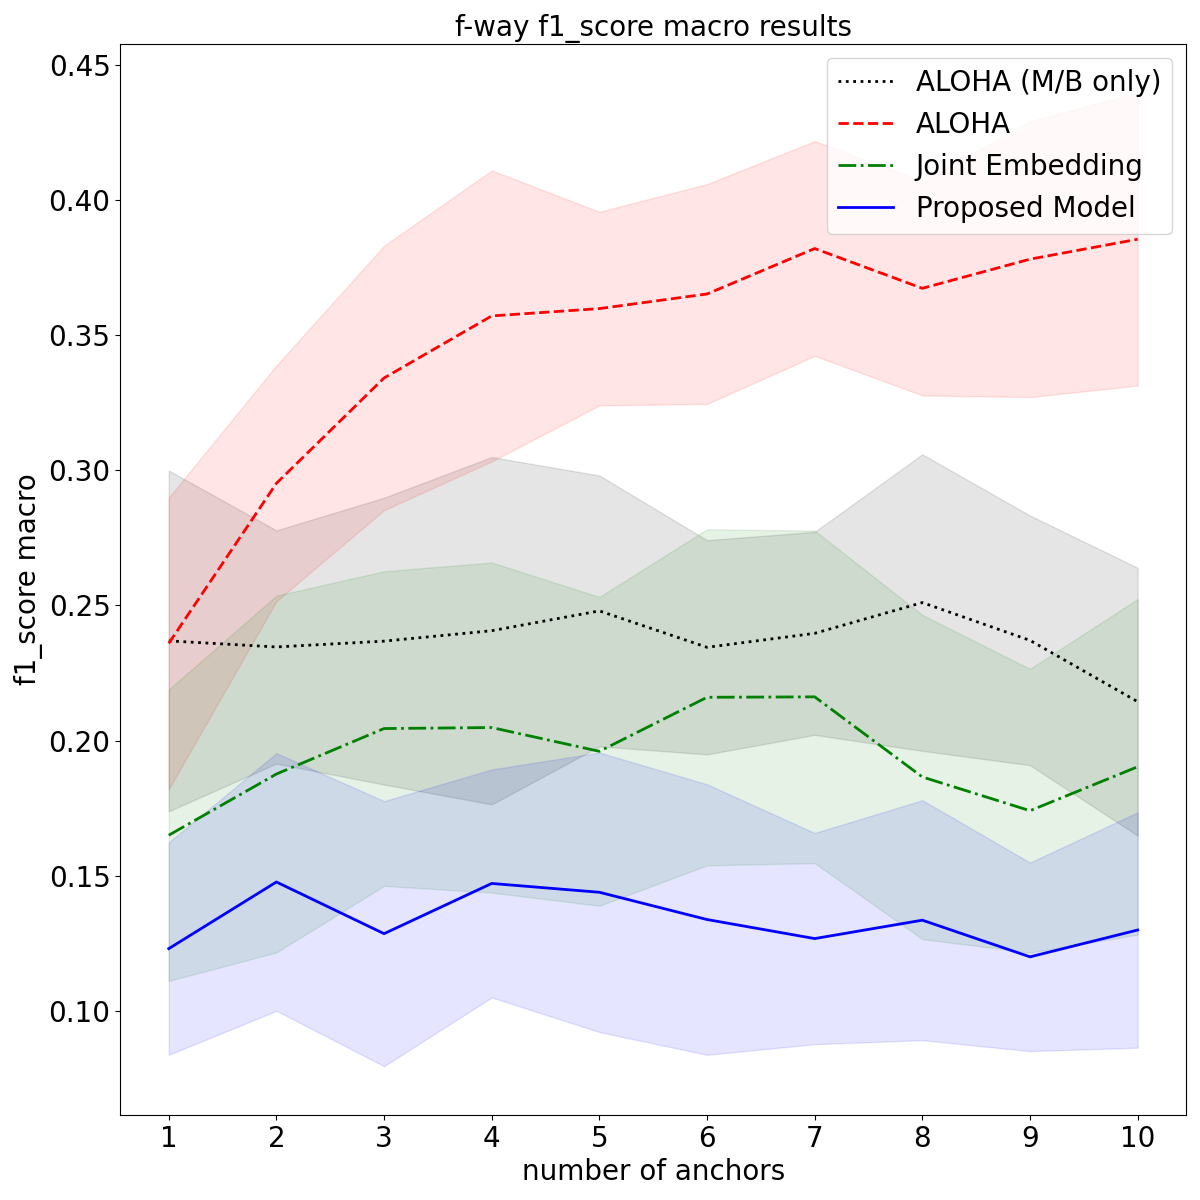
\includegraphics[width=0.6\textwidth]{./results/f1_score_macro_trends.png}
        \vspace*{-0.2cm}
        \caption[Family Prediction F1-score (Macro) Trends]{\textBF{F1-score (Macro) Trend} (varying the number of anchor samples used) resulting from the evaluation of the different models on the Malware Family Prediction task. The line represents the \textit{mean} F1-score (Macro), while the shaded region represents the \textit{standard deviation}. Statistics were computed over 15 evaluation of the same models with different query and anchor samples.}
        \label{fig:FScoreMacroTrends}
    \end{figure}
}

\newcommand{\allFScoreMicroTrends}{
    \begin{figure}[H]
        \vspace*{-0.5cm}
        \centering
        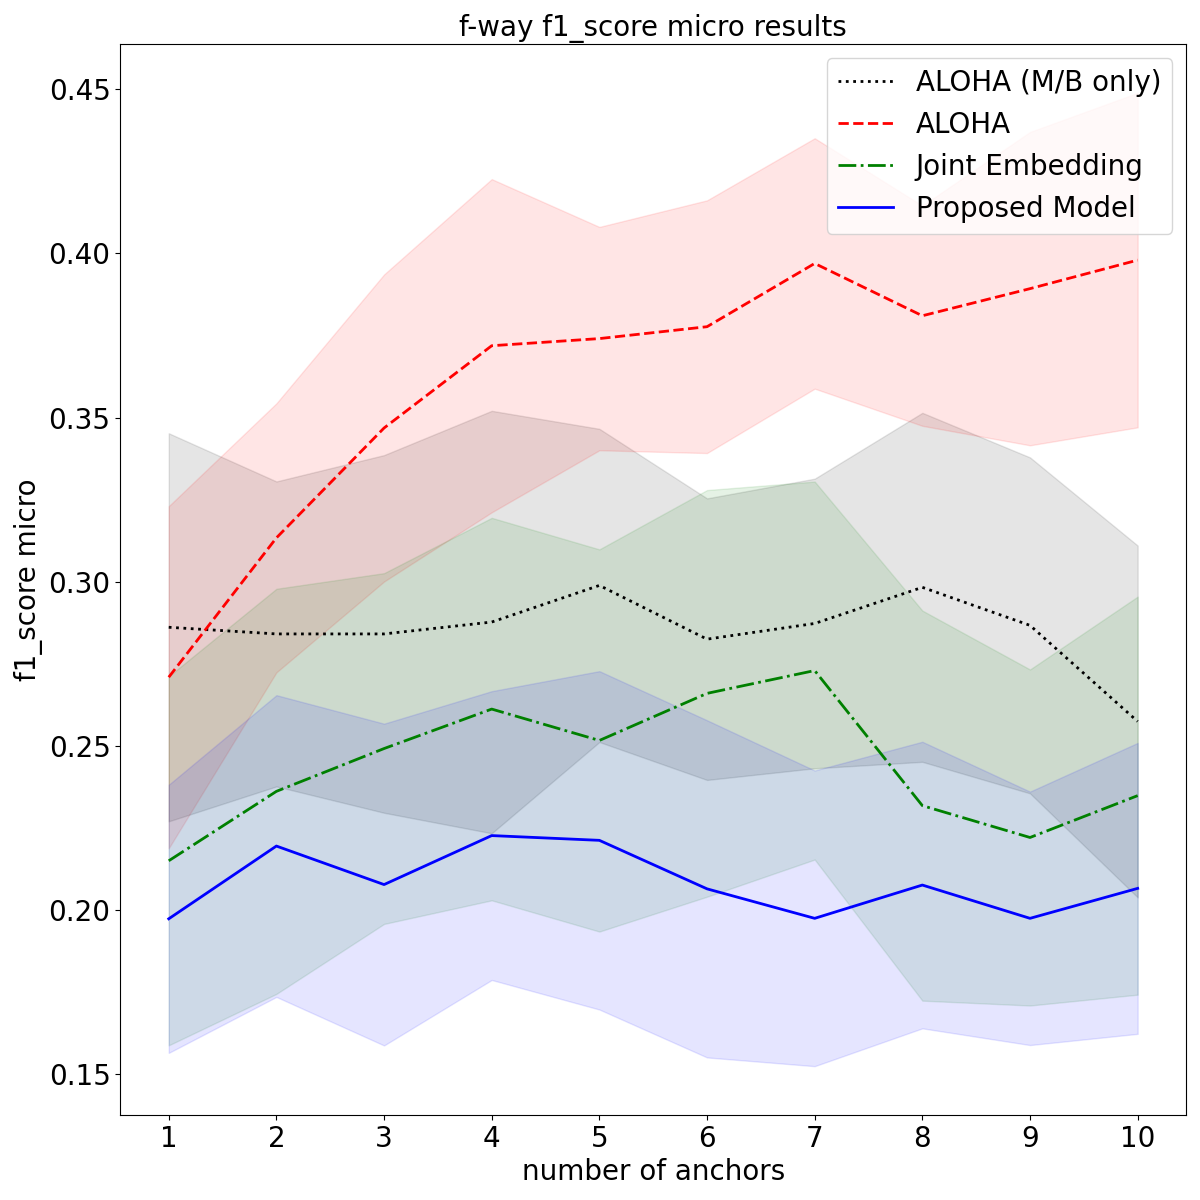
\includegraphics[width=0.6\textwidth]{./results/f1_score_micro_trends.png}
        \vspace*{-0.2cm}
        \caption[Family Prediction F1-score (Micro) Trends]{\textBF{F1-score (Micro) Trend} (varying the number of anchor samples used) resulting from the evaluation of the different models on the Malware Family Prediction task. The line represents the \textit{mean} F1-score (Micro), while the shaded region represents the \textit{standard deviation}. Statistics were computed over 15 evaluation of the same models with different query and anchor samples.}
        \label{fig:FScoreMicroTrends}
    \end{figure}
}

\newcommand{\allPrecisionMacroTrends}{
    \begin{figure}[H]
        \vspace*{-0.5cm}
        \centering
        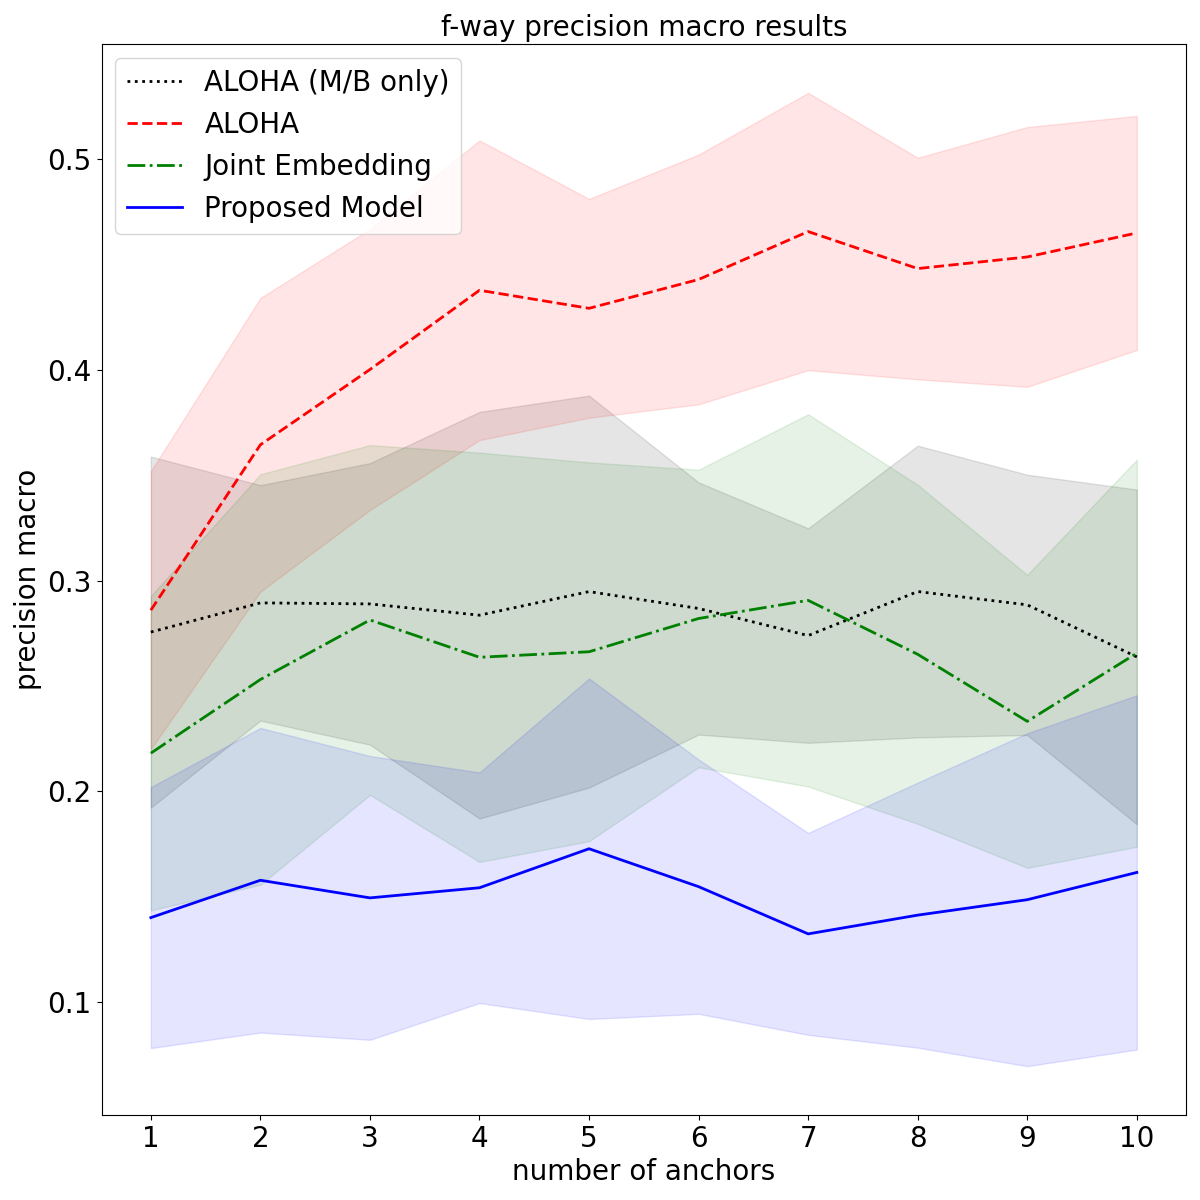
\includegraphics[width=0.6\textwidth]{./results/precision_macro_trends.png}
        \vspace*{-0.2cm}
        \caption[Family Prediction Precision (Macro) Trends]{\textBF{Precision (Macro) Trend} (varying the number of anchor samples used) resulting from the evaluation of the different models on the Malware Family Prediction task. The line represents the \textit{mean} Precision (Macro), while the shaded region represents the \textit{standard deviation}. Statistics were computed over 15 evaluation of the same models with different query and anchor samples.}
        \label{fig:PrecisionMacroTrends}
    \end{figure}
}

\newcommand{\allPrecisionMicroTrends}{
    \begin{figure}[H]
        \vspace*{-0.5cm}
        \centering
        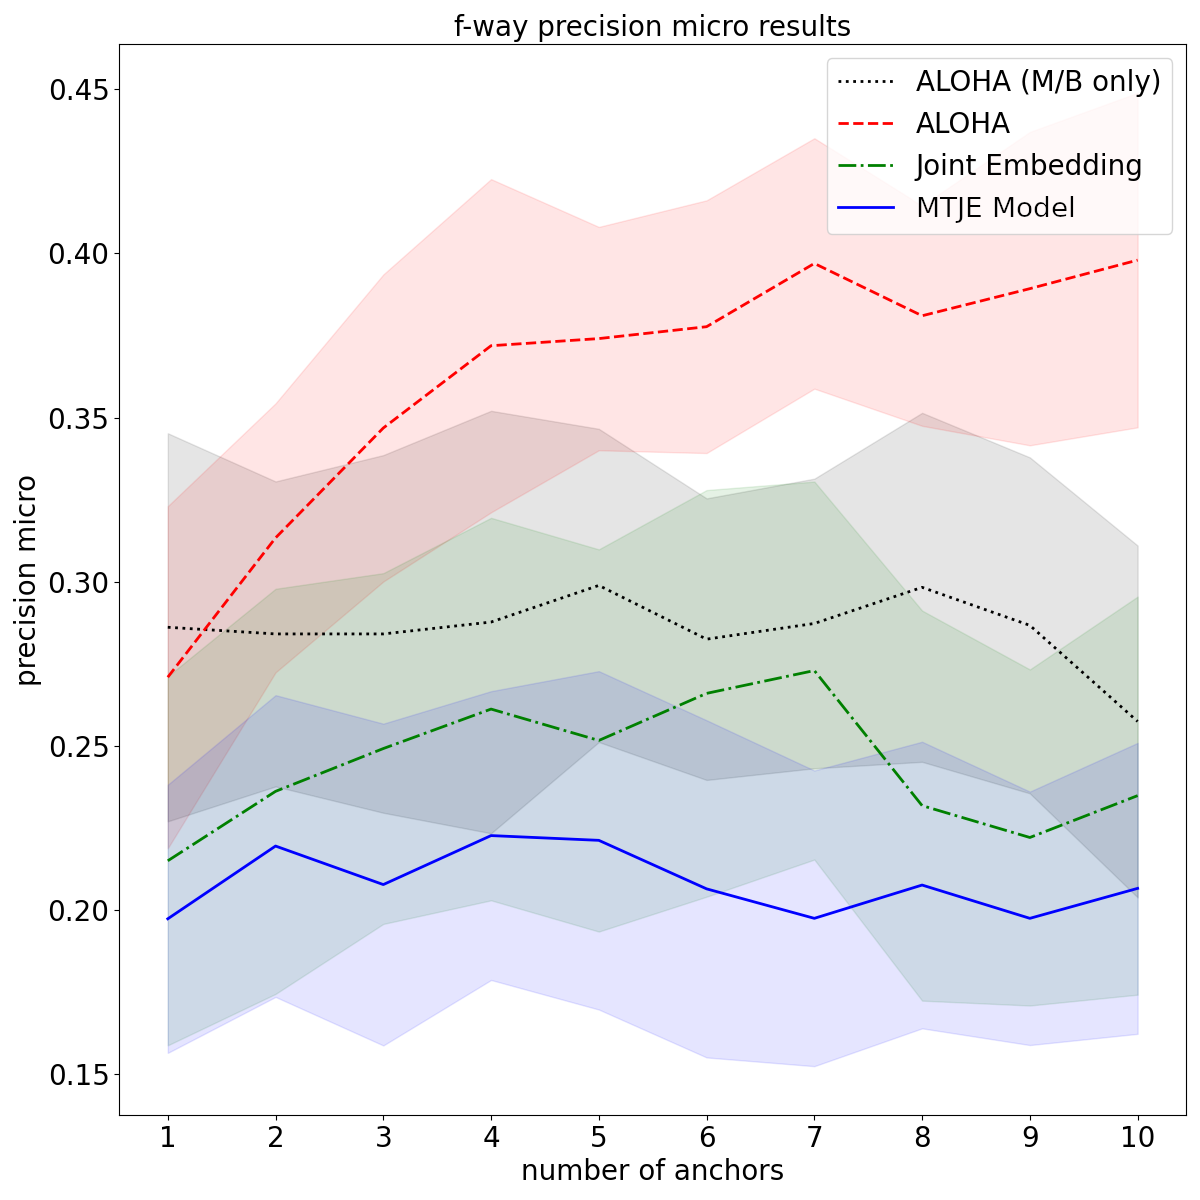
\includegraphics[width=0.6\textwidth]{./results/precision_micro_trends.png}
        \vspace*{-0.2cm}
        \caption[Family Prediction Precision (Micro) Trends]{\textBF{Precision (Micro) Trend} (varying the number of anchor samples used) resulting from the evaluation of the different models on the Malware Family Prediction task. The line represents the \textit{mean} Precision (Micro), while the shaded region represents the \textit{standard deviation}. Statistics were computed over 15 evaluation of the same models with different query and anchor samples.}
        \label{fig:PrecisionMicroTrends}
    \end{figure}
}

\newcommand{\allRecallScoreMacroTrends}{
    \begin{figure}[H]
        \vspace*{-0.5cm}
        \centering
        \includegraphics[width=0.6\textwidth]{./results/recall_score_macro_trends.png}
        \vspace*{-0.2cm}
        \caption[Family Prediction Recall (Macro) Trends]{\textBF{Recall (Macro) Trend} (varying the number of anchor samples used) resulting from the evaluation of the different models on the Malware Family Prediction task. The line represents the \textit{mean} Recall (Macro), while the shaded region represents the \textit{standard deviation}. Statistics were computed over 15 evaluation of the same models with different query and anchor samples.}
        \label{fig:RecallScoreMacroTrends}
    \end{figure}
}

\newcommand{\allRecallScoreMicroTrends}{
    \begin{figure}[H]
        \vspace*{-0.5cm}
        \centering
        \includegraphics[width=0.6\textwidth]{./results/recall_score_micro_trends.png}
        \vspace*{-0.2cm}
        \caption[Family Prediction Recall (Micro) Trends]{\textBF{Recall (Micro) Trend} (varying the number of anchor samples used) resulting from the evaluation of the different models on the Malware Family Prediction task. The line represents the \textit{mean} Recall (Micro), while the shaded region represents the \textit{standard deviation}. Statistics were computed over 15 evaluation of the same models with different query and anchor samples.}
        \label{fig:RecallScoreMicroTrends}
    \end{figure}
}

\newcommand{\allConfusionMatrixesMaxAcc}{
    \begin{figure}[H]
        \centering
        \begin{subfigure}[b]{0.475\textwidth}
            \centering
            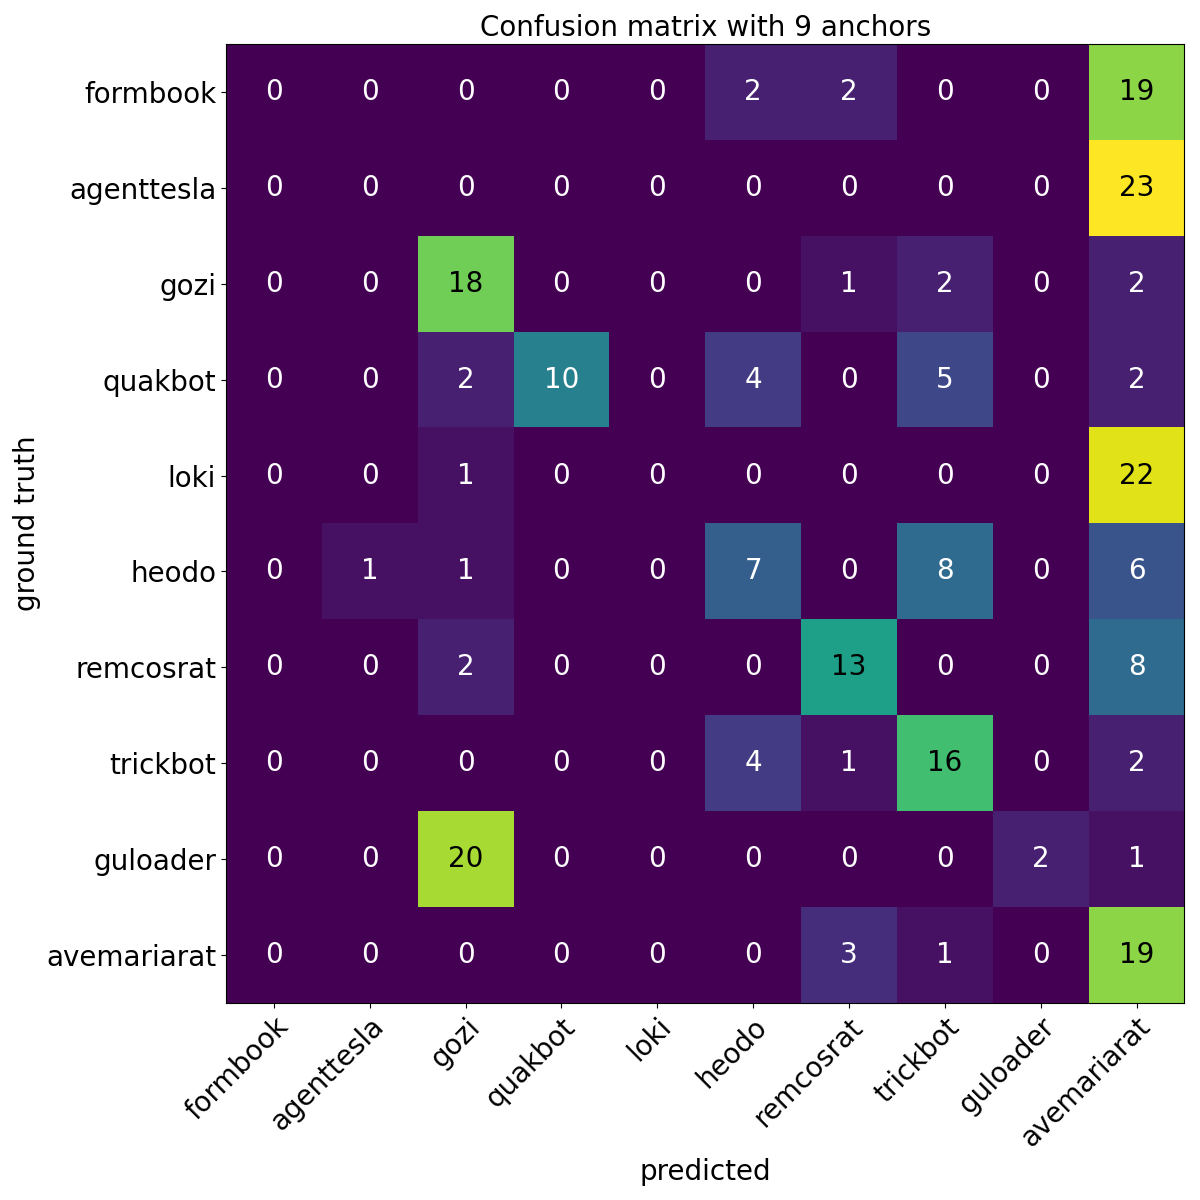
\includegraphics[width=\textwidth]{./results/conf_matrix_max_acc_alohaMB.png}
            \caption[]{{\small \textBF{ALOHA (M/B only)} implementation}}
            \label{fig:alohaConfMatrixMaxAcc}
        \end{subfigure}
        \hfill
        \begin{subfigure}[b]{0.475\textwidth}
            \centering
            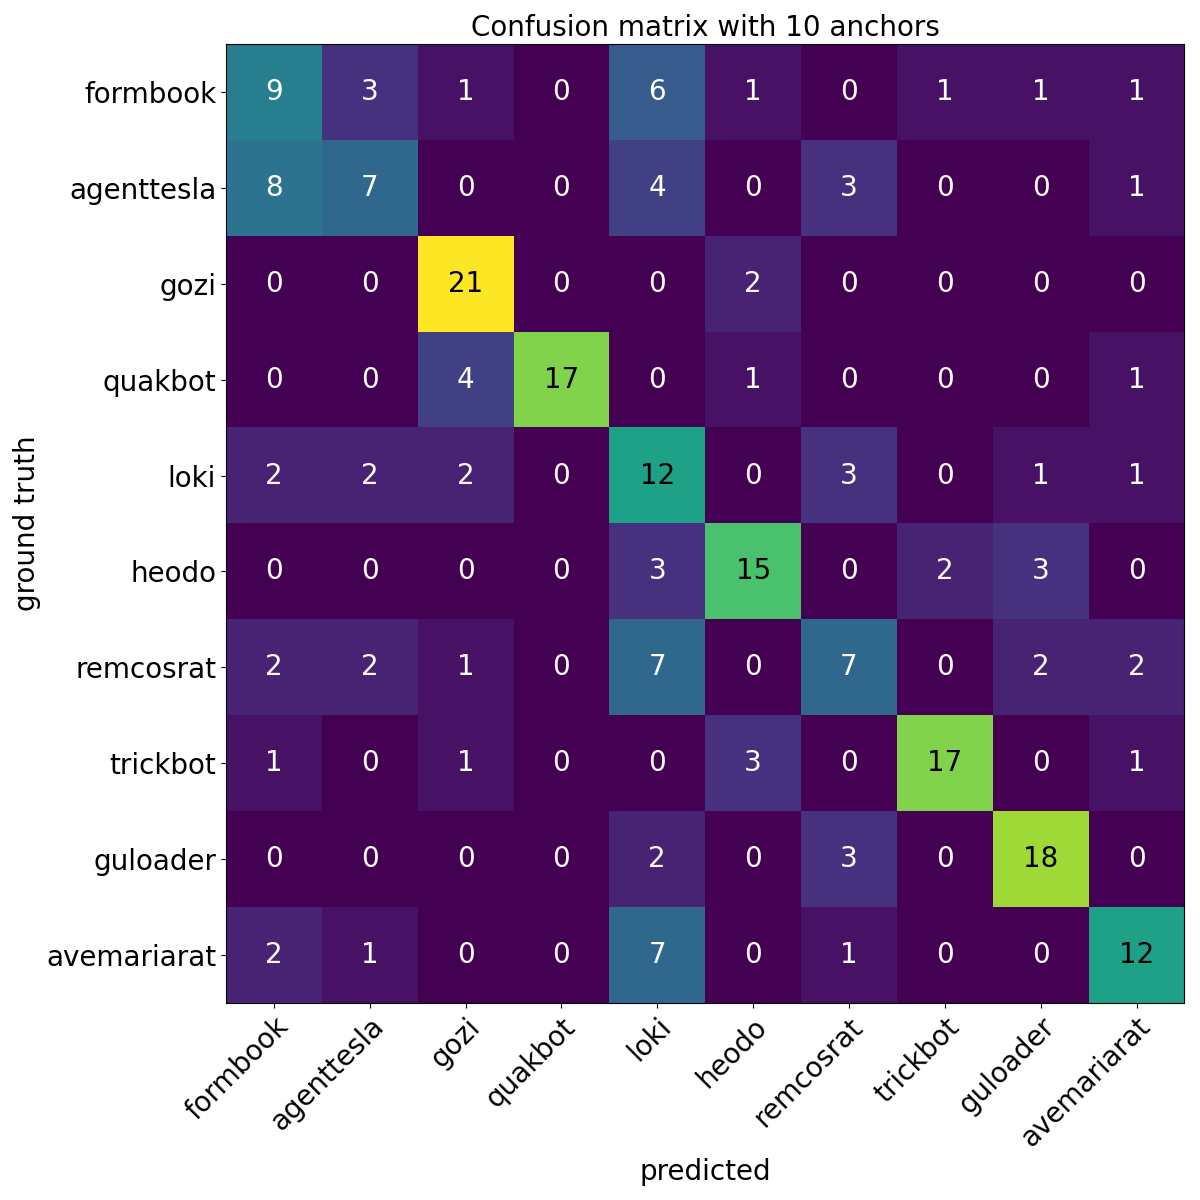
\includegraphics[width=\textwidth]{./results/conf_matrix_max_acc_aloha.png}
            \caption[]{{\small \textBF{ALOHA} implementation}}
            \label{fig:alohaMBConfMatrixMaxAcc}
        \end{subfigure}
        \vskip\baselineskip
        \begin{subfigure}[b]{0.475\textwidth}
            \centering
            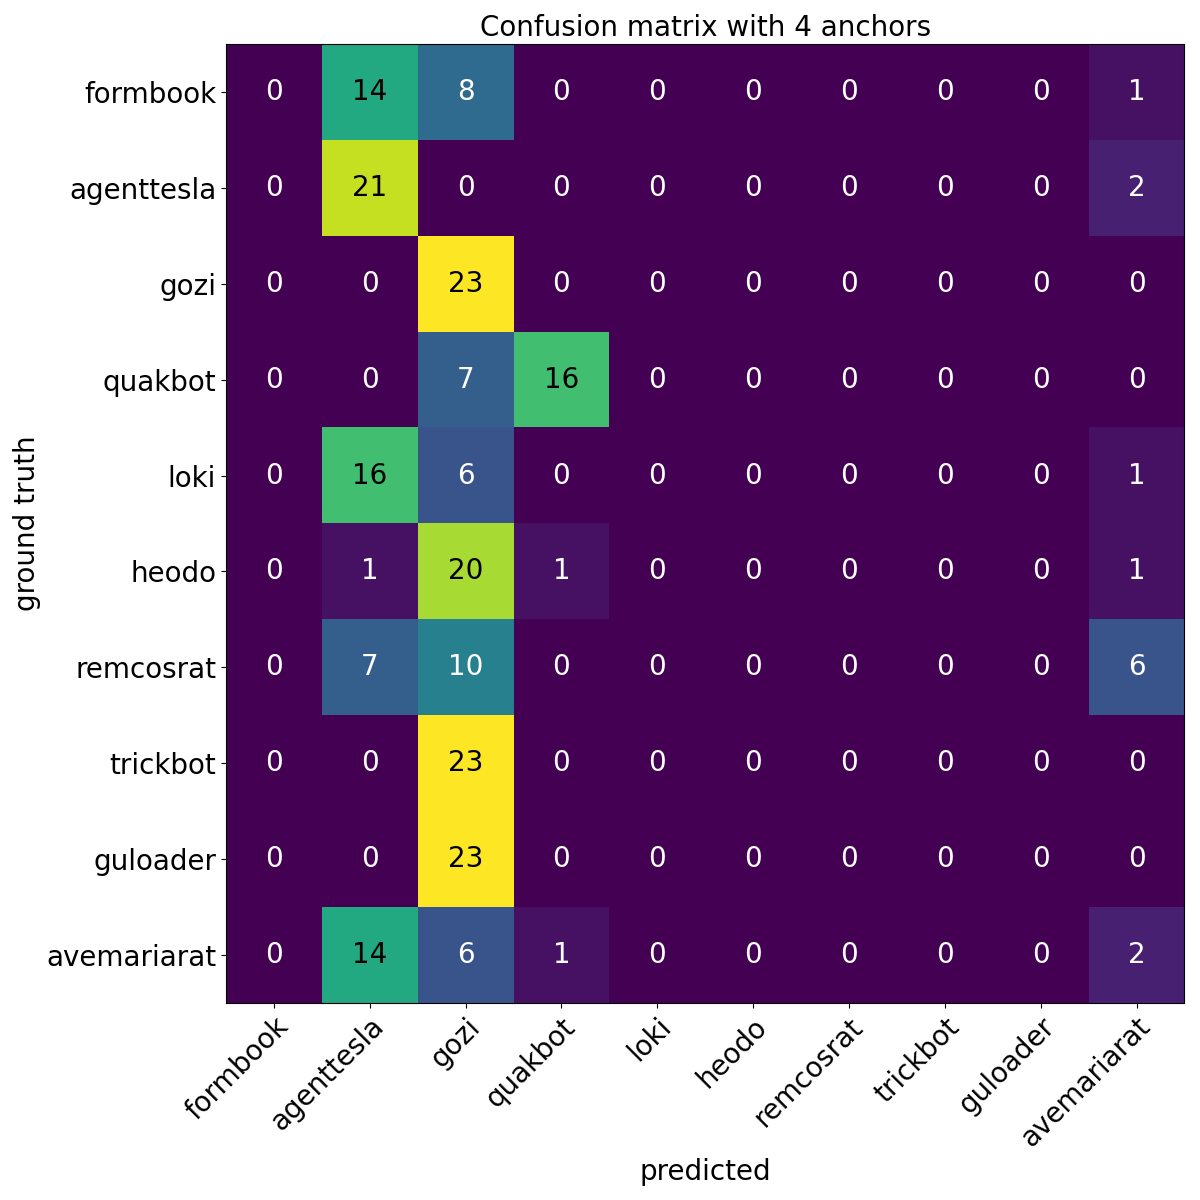
\includegraphics[width=\textwidth]{./results/conf_matrix_max_acc_jointEmbedding.png}
            \caption[]{{\small \textBF{Joint Embedding} implementation}}
            \label{fig:jointEmbeddingConfMatrixMaxAcc}
        \end{subfigure}
        \hfill
        \begin{subfigure}[b]{0.475\textwidth}
            \centering
            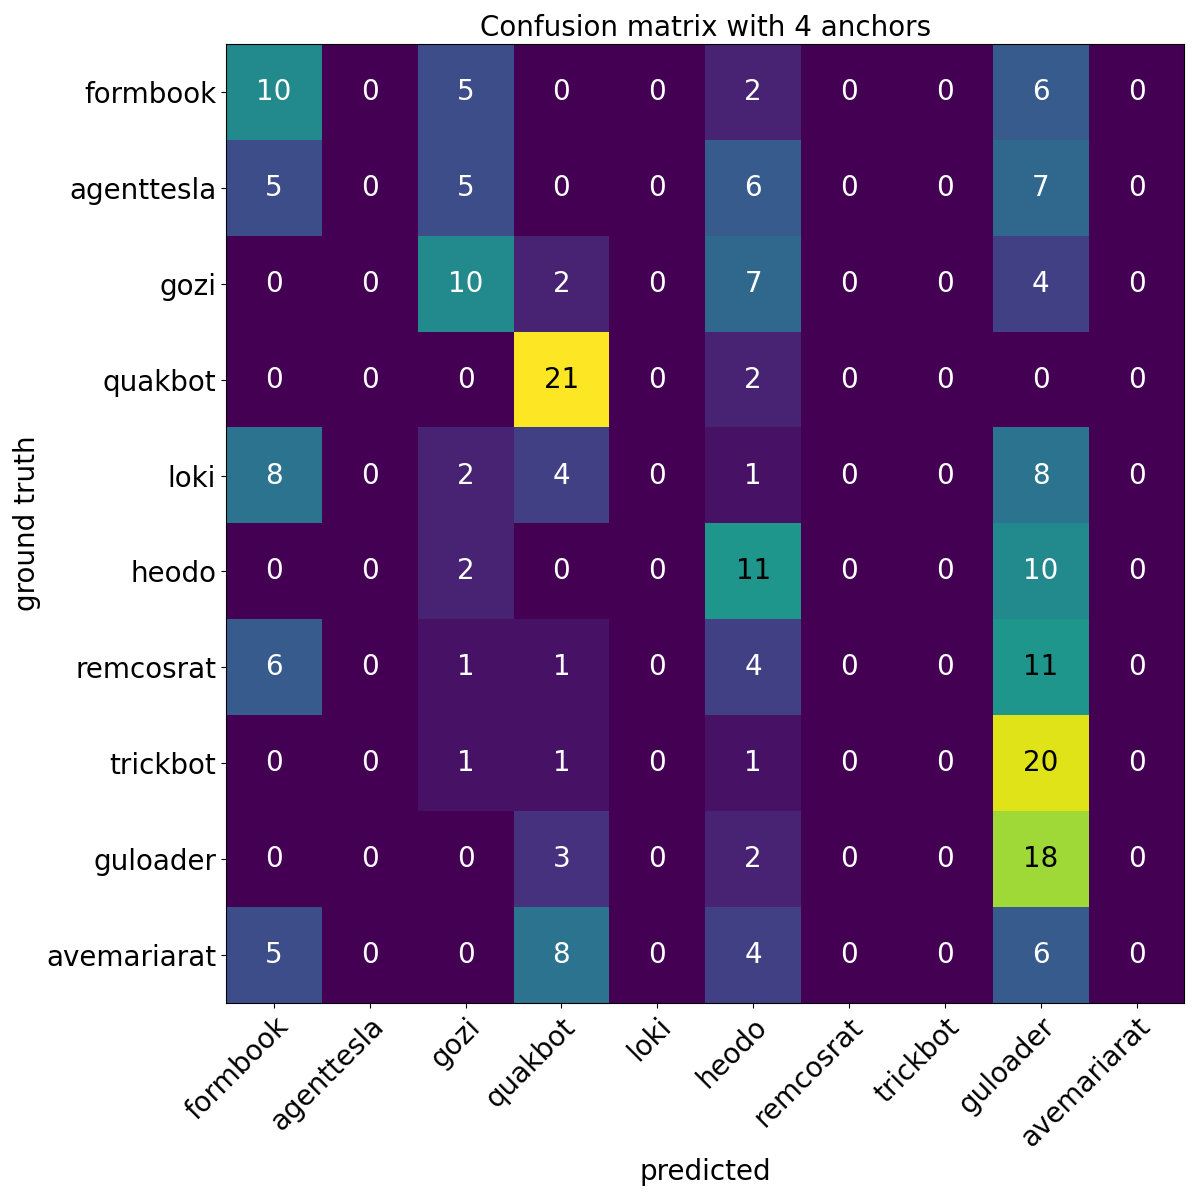
\includegraphics[width=\textwidth]{./results/conf_matrix_max_acc_proposedModel.png}
            \caption[]{{\small \textBF{Proposed Model} implementation}}
            \label{fig:proposedModelConfMatrixMaxAcc}
        \end{subfigure}
        \caption[Family Prediction Confusion Matrixes (Max Accuracy)]{\textBF{Confusion Matrix} corresponding to the best prediction when using the number $k$ of anchors which produced the overall best accuracy, resulting from the evaluation of the different models on the Malware Family Prediction task.}
        \label{fig:ConfusionMatrixesMaxAcc}
    \end{figure}
}

\newcommand{\allConfusionMatrixesMinAcc}{
    \begin{figure}[H]
        \centering
        \begin{subfigure}[b]{0.475\textwidth}
            \centering
            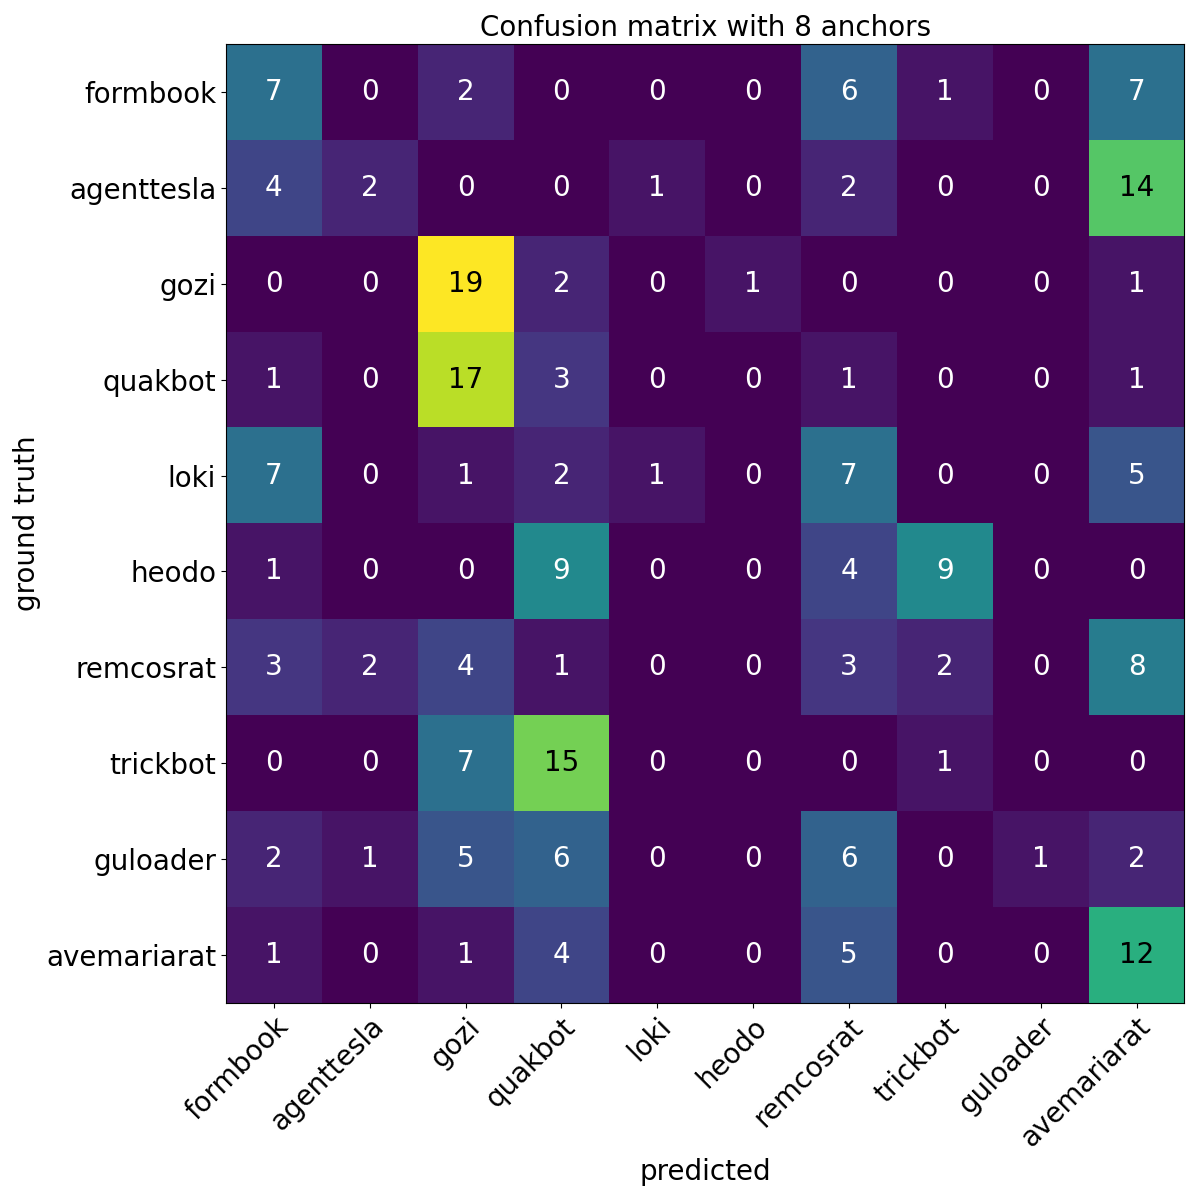
\includegraphics[width=\textwidth]{./results/conf_matrix_min_acc_alohaMB.png}
            \caption[]{{\small \textBF{ALOHA (M/B only)} implementation}}
            \label{fig:alohaConfMatrixMinAcc}
        \end{subfigure}
        \hfill
        \begin{subfigure}[b]{0.475\textwidth}
            \centering
            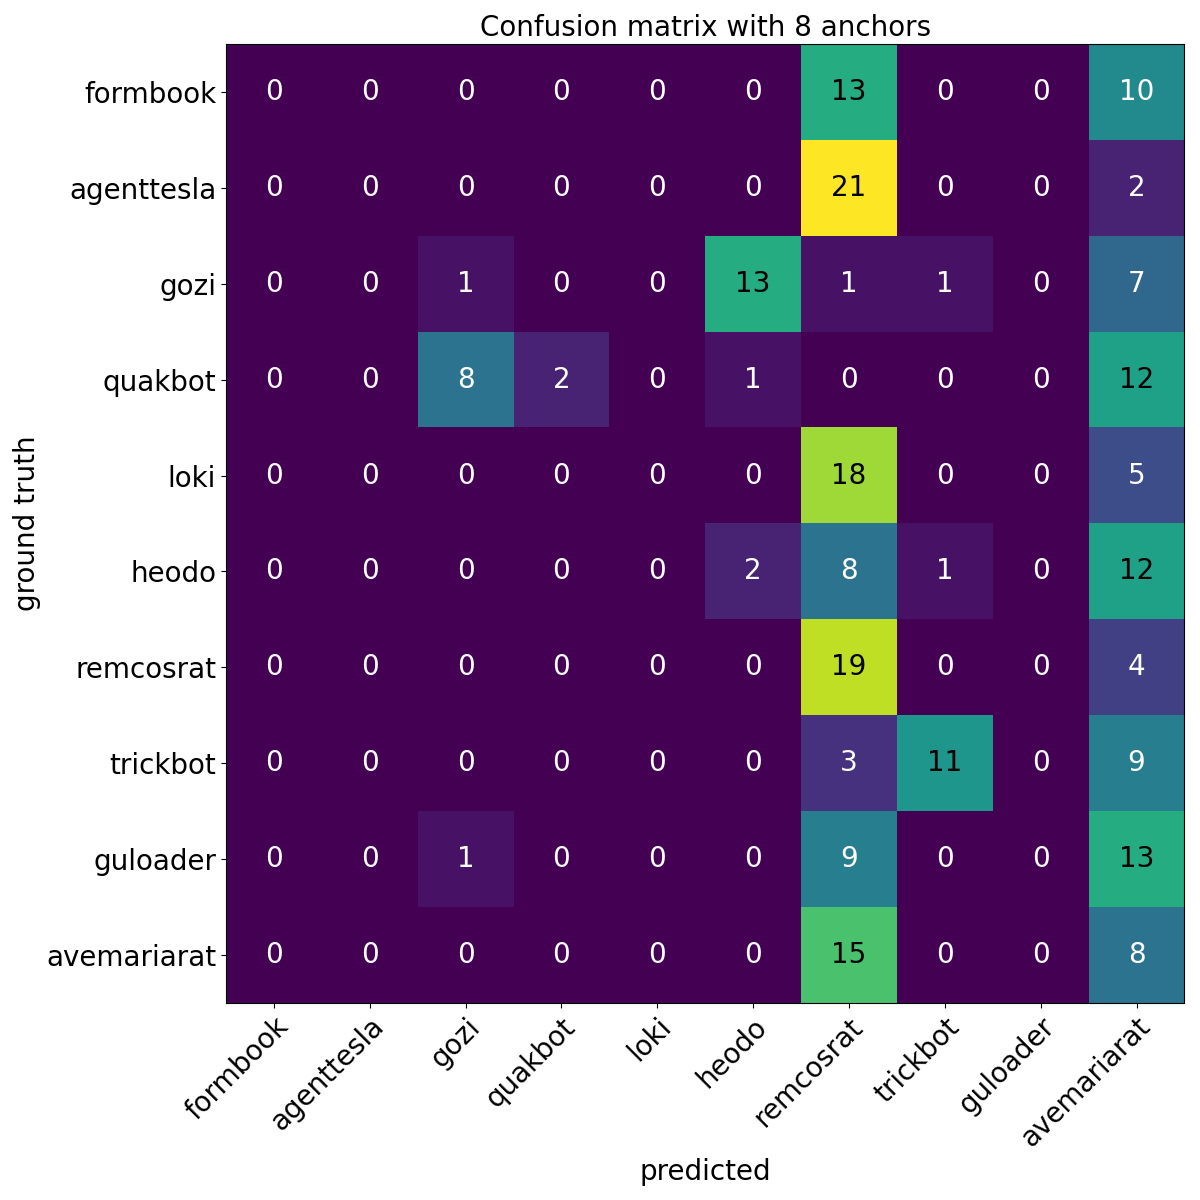
\includegraphics[width=\textwidth]{./results/conf_matrix_min_acc_aloha.png}
            \caption[]{{\small \textBF{ALOHA} implementation}}
            \label{fig:alohaMBConfMatrixMinAcc}
        \end{subfigure}
        \vskip\baselineskip
        \begin{subfigure}[b]{0.475\textwidth}
            \centering
            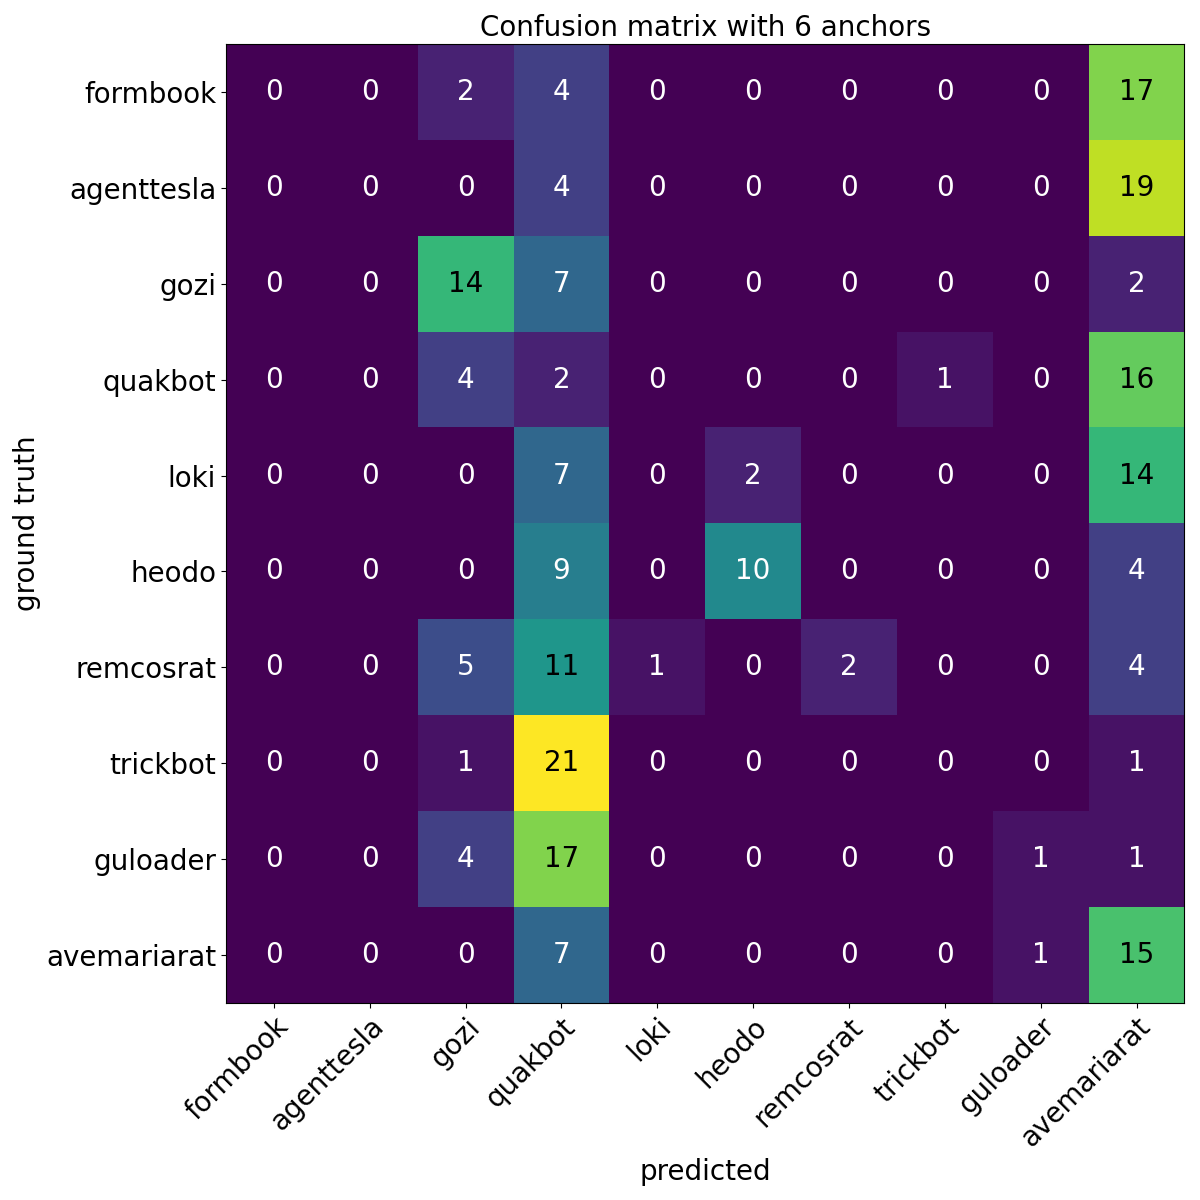
\includegraphics[width=\textwidth]{./results/conf_matrix_min_acc_jointEmbedding.png}
            \caption[]{{\small \textBF{Joint Embedding} implementation}}
            \label{fig:jointEmbeddingConfMatrixMinAcc}
        \end{subfigure}
        \hfill
        \begin{subfigure}[b]{0.475\textwidth}
            \centering
            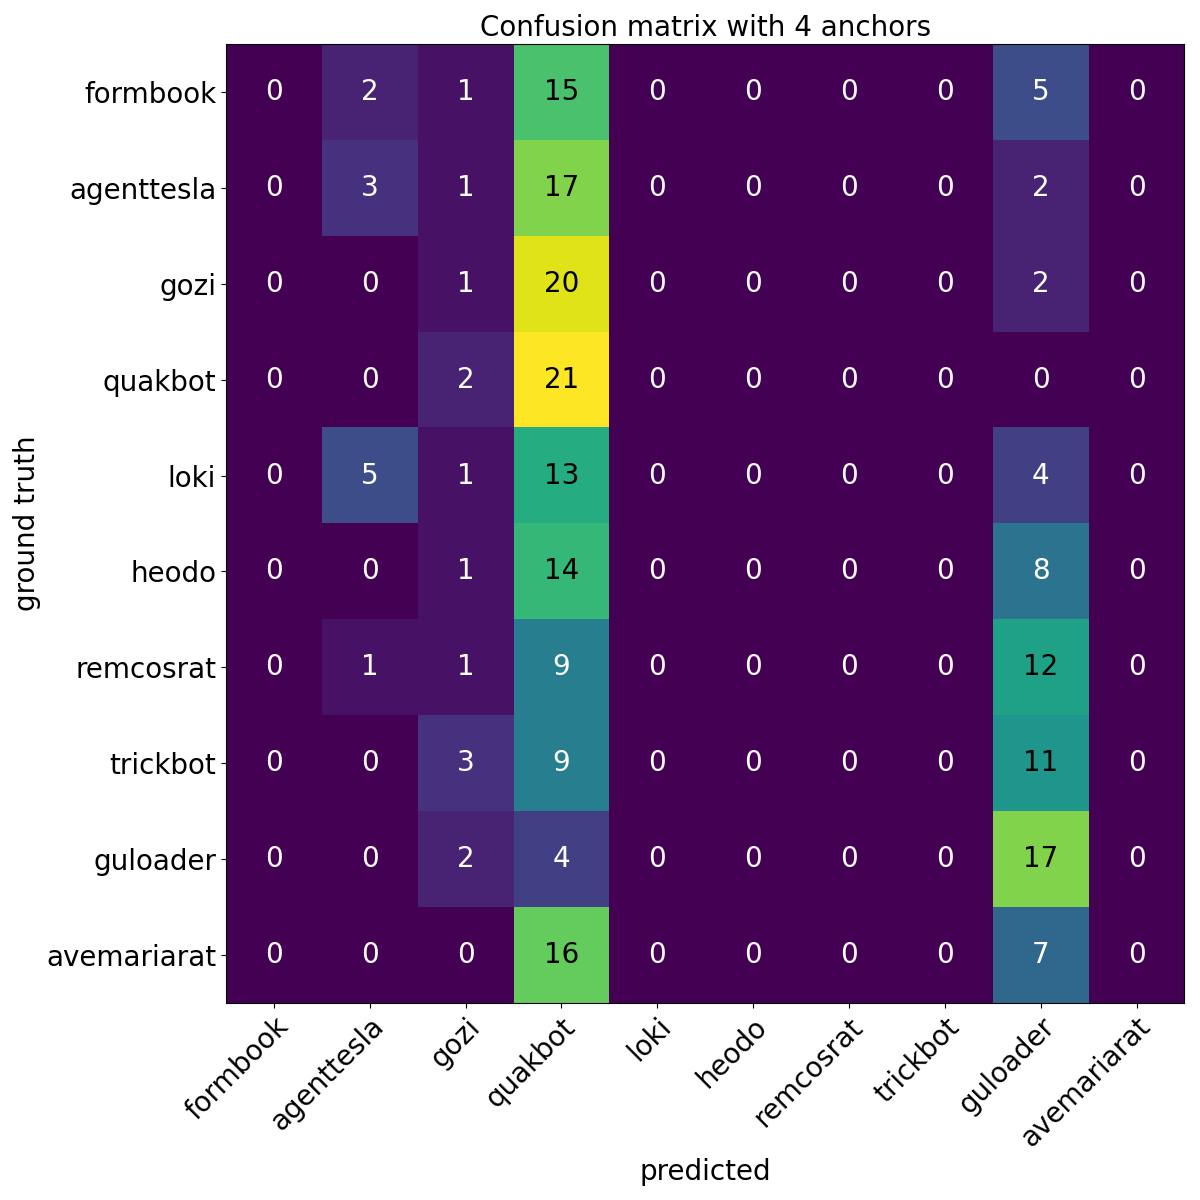
\includegraphics[width=\textwidth]{./results/conf_matrix_min_acc_proposedModel.png}
            \caption[]{{\small \textBF{Proposed Model} implementation}}
            \label{fig:proposedModelConfMatrixMinAcc}
        \end{subfigure}
        \caption[Family Prediction Confusion Matrixes (Min Accuracy)]{\textBF{Confusion Matrix} corresponding to the best prediction when using the number $k$ of anchors which produced the overall worst accuracy, resulting from the evaluation of the different models on the Malware Family Prediction task.}
        \label{fig:ConfusionMatrixesMinAcc}
    \end{figure}
}

